\documentclass[11pt]{article}
\usepackage[margin=1in, top=1in]{geometry}
\usepackage[all]{nowidow}
\usepackage[hyperfigures=true, hidelinks, pdfhighlight=/N]{hyperref}
\usepackage[separate-uncertainty=true, group-digits=true]{siunitx}
\usepackage{graphicx,amsmath,physics,tabto,float,amssymb,pgfplots,verbatim,tcolorbox}
\usepackage{listings,xcolor,subfig,caption,import,wrapfig,enumitem}
\usepackage[version=4]{mhchem}
\usepackage[noabbrev]{cleveref}
\newcommand{\creflastconjunction}{, and\nobreakspace}
\newcommand{\mb}[1]{\mathbf{#1}}
\definecolor{stringcolor}{HTML}{C792EA}
\definecolor{codeblue}{HTML}{2162DB}
\definecolor{commentcolor}{HTML}{4A6E46}
\captionsetup{font=small, belowskip=0pt}
\lstdefinestyle{appendix}{
    basicstyle=\ttfamily\footnotesize,commentstyle=\color{commentcolor},keywordstyle=\color{codeblue},
    stringstyle=\color{stringcolor},showstringspaces=false,numbers=left,upquote=true,captionpos=t,
    abovecaptionskip=12pt,belowcaptionskip=12pt,language=Python,breaklines=true,frame=single}
\lstdefinestyle{inline}{
    basicstyle=\ttfamily\footnotesize,commentstyle=\color{commentcolor},keywordstyle=\color{codeblue},
    stringstyle=\color{stringcolor},showstringspaces=false,numbers=left,upquote=true,frame=tb,
    captionpos=b,language=Python}
\renewcommand{\lstlistingname}{Appendix}
\pgfplotsset{compat=1.17}

\begin{document}

\begin{center}
    \textbf{CP Test 1}\hspace{1.5in}\textbf{KDSMIL001}\hspace{1.5in}\textbf{14-05-2022}
\end{center}
\rule{\textwidth}{1pt}

\begin{enumerate}
    \item \begin{enumerate}
        \item We begin, when integrating using Gauss-Laguerre quadrature, by transforming the integrals in question,
        \begin{equation}
            I = \frac{\int_0^\infty (x^4 +1)xe^{-\sqrt{4x^2 +1}}dx}{\int_0^\infty xe^{-\sqrt{4x^2 +1}}dx}
            \label{eqn:Q1Integral}
        \end{equation}
        into ones of the form
        \begin{equation}
            \int_0^\infty f(x)e^{-x}.
            \label{eqn:GaussLaguerreGenForm}
        \end{equation}
        We begin with the numerator, which we will call $I_N$. Choosing the substitution $w=\sqrt{4x^2+1}$, we get
        \begin{equation*}
            x=\sqrt{\frac{w^2-1}{4}}, \;\;\; x^4+1=\left(\frac{w^2-1}{4}\right)^2+1, \;\;\; dx=\frac{w}{2\sqrt{w^2-1}}dw 
        \end{equation*}
        Then we find 
        \begin{align*}
            I_N&=\int_1^\infty \frac{w}{2\sqrt{w^2-1}} \left(\left(\frac{w^2-1}{4}\right)^2+1\right) \sqrt{\frac{w^2-1}{4}} e^{-w} dw\\
            &=\int_0^\infty \frac{w}{4}\left(\left(\frac{w^2-1}{4}\right)^2+1\right)e^{-w} dw
        \end{align*}
        Using another substitution, $x=w-1$, we can see 
        \begin{equation}
            I_N = \int_0^\infty \frac{x+1}{4}\left(\left(\frac{x^2+2x}{4}\right)^2+1\right)e^{-x-1}
            \label{eqn:q1iNumerator}
        \end{equation}
        where we easily identify
        \begin{equation}
            f_N(x) = \frac{x+1}{4e}\left(\left(\frac{x^2+2x}{4}\right)^2+1\right).
            \label{eqn:q1iFN}
        \end{equation}
        For the denominator, we use the same two substitutions, finding
        \begin{align}
            I_D &= \int_0^\infty xe^{-\sqrt{4x^2 +1}}dx \nonumber\\
            &=\int_1^\infty \frac{w}{4}e^{-w} dw \nonumber\\
            &=\int_0^\infty \frac{x+1}{4e}e^{-x} dx \label{eqn:q1iDenominator}\\
            \implies f_D(x) &= \frac{x+1}{4e}. \label{eqn:q1iFD}
        \end{align}
        We can then use Gauss-Laguerre quadrature to find these integrals:
        \begin{align}
            I_N &\approx \sum_{i=1}^n f_N(x_i)w_i \label{eqn:GLNumerator}\\
            I_D &\approx \sum_{i=1}^n f_D(x_i)w_i \label{eqn:GLDenominator}
        \end{align}
        where the $x_i$ are the roots of the $n$-th order Laguerre polynomial, and $w_i$ are the respective weights. These can be found using \texttt{np.polynomial.laguerre.laggauss(n)}.\\
        Using a 16-th order Laguerre polynomial, we find $I \approx 10.250000000000082$, which is pretty bang on $10.25$.

        \item For a Monte Carlo integration method, we choose the Metropolis method, as the integral in \cref{eqn:Q1Integral} is of the form
        \begin{equation}
            I = \frac{\int p(x)f(x)dx}{\int p(x)dx}.
            \label{eqn:MetropolisGeneralForm}
        \end{equation}
        We can identify $f(x)=x^4+1$, and thus we need to sample according to 
        \begin{equation}
            p(x) = xe^{-\sqrt{4x^2 +1}}.
            \label{eqn:q1iiProbDist}
        \end{equation}
        Using the Metropolis method allows us to not have to normalise this $p(x)$, which is nice as the integral of it is a bit ugly. It is also effective as we need to generate this distribution on a semi-infinite interval, which Metropolis has no problems with.\\
        
        To begin with, we generate $N_0=\num[]{500000}$ points $x_i$, according to $p(x)$ using the Metropolis random walk/Markov chain method, with $\Delta=2$ for an acceptance rate of about 45\%. In order to avoid correlation between points we compute the autocorrelation function 
        \begin{equation}
            C(j) = \frac{\langle x_{i+j}x_i\rangle - \langle x_i \rangle^2}{\langle x_i^2 \rangle - \langle x_i \rangle^2}
            \label{eqn:Autocorrelation}
        \end{equation}
        for a range of $j$ values, and find the first $j$ for which $C(j)< 0.01$. \Cref{fig:correlation} shows the results.

        
        This tells us how many numbers in the Markov chain to skip each time we choose one to be part of our final distribution. We also need to consider the starting values, as the method goes through a transient phase before equilibrating. To find how many numbers to chop off the start, we can find the moving average of the $N_0$ generated values, and see when it begins to level off. \Cref{fig:equilibrium} shows the results.\\
        By inspection, we can see it levels off at around \num[]{20000} points, so we choose to cut off the first \num[]{20000} points. Doing this and skipping every 17 points leaves us with around \num[]{28000} points in our distribution. \Cref{fig:histogram} shows the resulting histogram, along with the expected distribution. \\
        We can test the "randomness" of these numbers by plotting a scatter plot of neighbouring points and looking for any regularities, or correlations. We can see in \cref{fig:randomness} that there is no regularity to be seen. \\
        With these randomly generated numbers $x_i$, we can finally compute $I$ in \cref{eqn:Q1Integral} using
        \begin{equation}
            I \approx \frac{1}{N}\sum_{i=1}^N f(x_i)
            \label{eqn:MetropolisIntegration}
        \end{equation}
        where $N\sim\num[]{28000}$. We find $I\approx \num[]{10.48 \pm 0.29}$. This uncertainty is calculated using 
        \begin{equation}
            u(I) = \frac{\sigma}{\sqrt N} = \frac{\sqrt{\langle f^2 \rangle - \langle f \rangle^2}}{\sqrt N}.
            \label{eqn:uncertainty}
        \end{equation}

        \item Calculating the integral $I$ in \cref{eqn:Q1Integral} in Mathematica, we find the exact result to be $\frac{41}{4}=10.25$. We see that Gauss-Laguerre worked very well, producing the result to an accuracy that could likely be waved away with computer precision. We also see that the Monte Carlo method result agrees with the exact and Gauss-Laguerre results.
        
        \begin{figure}[H]
            \begin{center}
                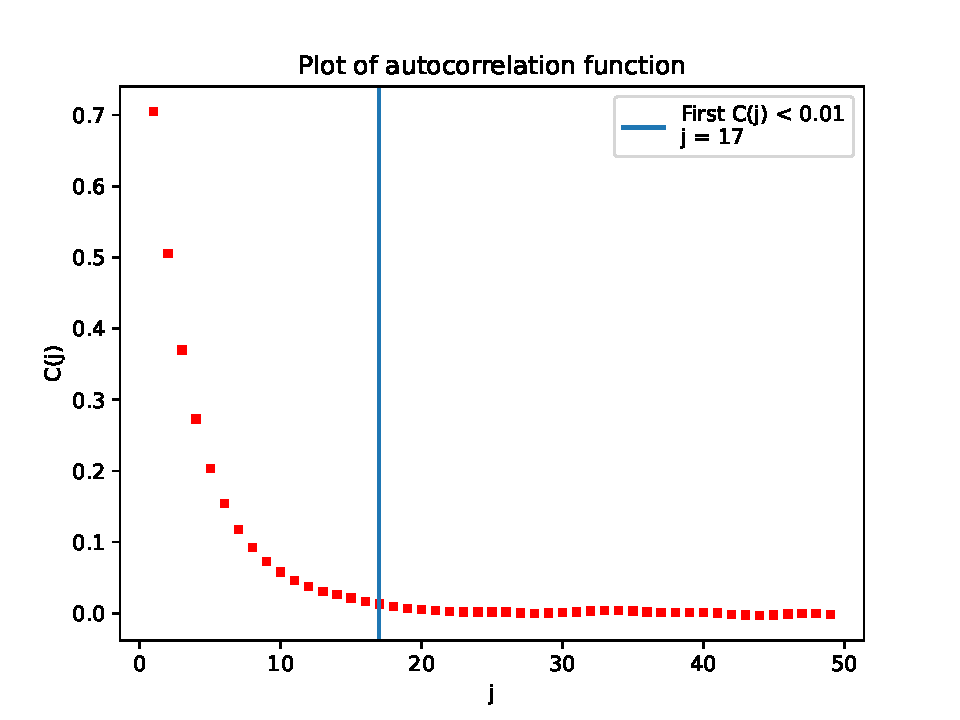
\includegraphics[width=.65\textwidth]{Plots/correlation.pdf}
                \caption{Plot of the autocorrelation function for the $N_0$ generated values, giving us $C(j=17)$ as the first value $< 0.01$. }
                \label{fig:correlation}
            \end{center}
        \end{figure}

        \begin{figure}[H]
            \begin{center}
                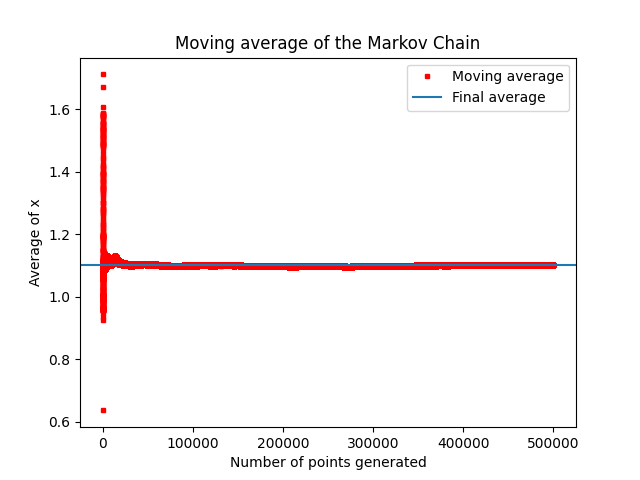
\includegraphics[width=.65\textwidth]{Plots/equilibrium.png}
                \caption{Plot of the moving average of the $N_0$ points in the generated Markov chain, along with the final average, to see when the moving average begins to level off.}
                \label{fig:equilibrium}
            \end{center}
        \end{figure}
        
        \begin{figure}[H]
            \begin{center}
                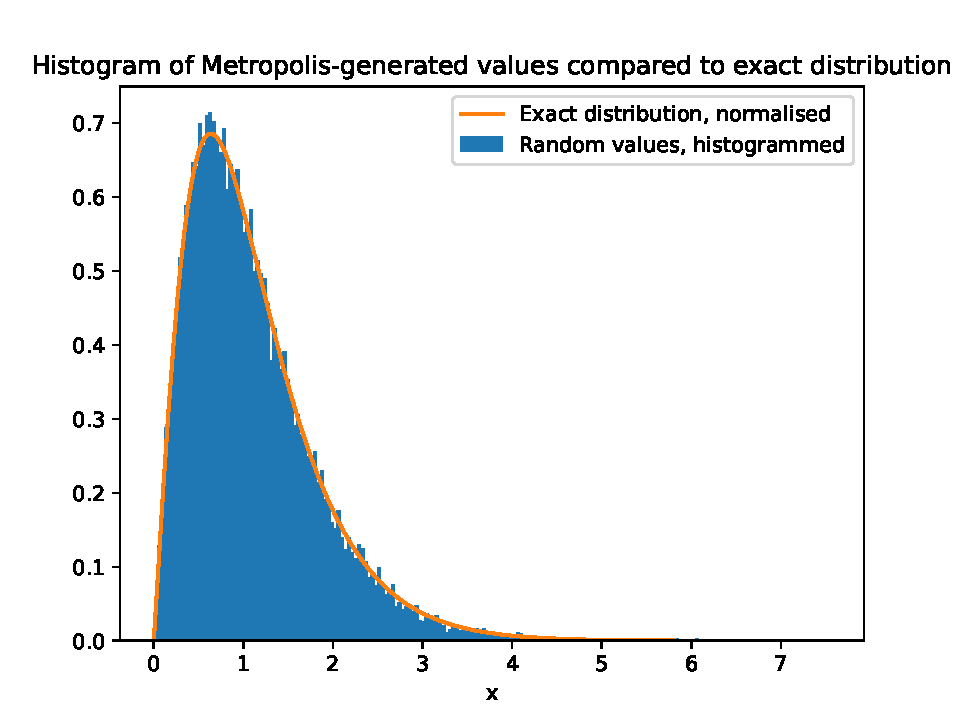
\includegraphics[width=.65\textwidth]{Plots/histogram.pdf}
                \caption{Histogram of the $x$-values calculated using the Metropolis method, distributed according to \cref{eqn:q1iiProbDist}, along with the exact distribution. Note that the histogram is normalised to 1 over the interval shown, while $p(x)$ is normalised over the semi-infinite interval, so there may be some discrepancies.}
                \label{fig:histogram}
            \end{center}
        \end{figure}

        \begin{figure}[H]
            \begin{center}
                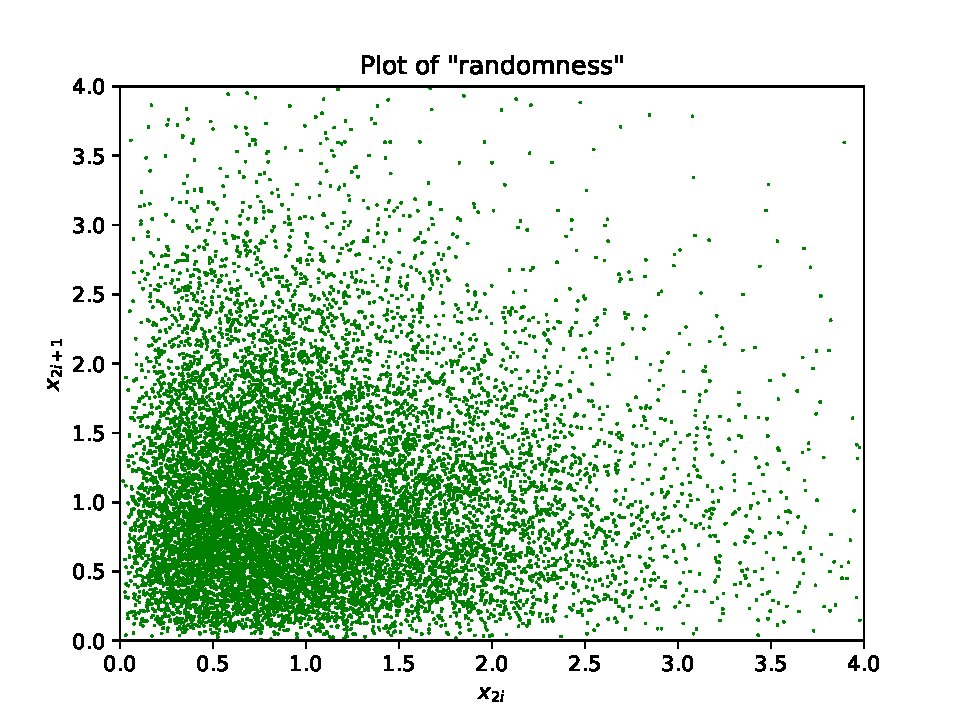
\includegraphics[width=.65\textwidth]{Plots/randomness.pdf}
                \caption{Plot of the "randomness" of the numbers generated with the Metropolis method. Plotted is every second point and its corresponding neighbour in front if it. Note that this is a cropped version of the entire plot, to better show off the area where most of the points lie. Only a few outliers have been cropped out.}
                \label{fig:randomness}
            \end{center}
        \end{figure}

    \end{enumerate}

    \item We aim to solve the boundary value problem
    \begin{equation}
        \frac{d^2V}{dr^2}+\frac{2}{r}\frac{dV}{dr}=0
        \label{eqn:Laplace}
    \end{equation}
    with BCs $V(r=\SI{1}{\metre})=\SI{20}{\volt}$ and $V(r=\SI{3}{\metre})=\SI{55}{\volt}$. Since this is a linear, second order ODE, we can simply use the linear finite difference scheme to solve it. To do this, we first approximate the derivatives as finite differences. Using the notation $V_i=V(r_i)$, and constructing a grid with spacing $\Delta r$, we have
    \begin{align*}
        0 &= \frac{V_{i-1} - 2V_i + V_{i+1}}{\Delta r^2} + \frac{2}{r_i}\frac{V_{i+1} - V_{i-1}}{2\Delta r} \\
        &= V_{i-1}\underbrace{\left(1-\frac{\Delta r}{r_i}\right)}_\alpha -2V_i+V_{i+1}\underbrace{\left(1+\frac{\Delta r}{r_i}\right)}_\beta \\
        &= \alpha V_{i-1} -2V_i +\beta V_{i+1}
    \end{align*}
    We can now consider this problem to be a matrix equation $A \mb{V}=\mb{w}$ where $A$ is a tridiagonal matrix, $\mb{V}$ is the $V_i$'s that make up the solution to \cref{eqn:Laplace}, and $\mb{w}$ is effectively the RHS of the ODE. \\
    If we split our interval into $N+2$ points, going from $i=0$ to $i=N+1$, we can construct our matrix equation:

    \begin{equation}
        \begin{pmatrix}
            -2 & \beta & 0 & \cdots & 0 \\
            \alpha & -2 & \beta & \cdots & 0 \\
            0 & \ddots & \ddots & \ddots & \vdots \\
            \vdots & \cdots & \alpha & -2 & \beta \\
            0 & \cdots & \cdots & \alpha & -2 
        \end{pmatrix}
        \begin{pmatrix}
            V_1 \\
            V_2 \\
            \vdots \\
            V_{N-1} \\
            V_N
        \end{pmatrix}
        =
        \begin{pmatrix}
            -\alpha V_0 \\
            0 \\
            \vdots \\
            0 \\
            -\beta V_{N+1}
        \end{pmatrix}
        \label{eqn:matrixEqn}
    \end{equation}

    What is important to note here is the appearance of our BCs in $\mb{w}$, on the RHS. This is due to a quirk in how the matrix gets constructed, but allows us to solve this system exactly, in one step, as we know all of $A$ and $\mb{w}$ explicitly, so we can just invert $A$. Doing this with \texttt{np.linalg.solve} and tacking on the two BCs, as this method does not return them in $\mb{V}$, we find the plot in \cref{fig:LaplaceFD}.

    \begin{figure}[h]
        \begin{center}
            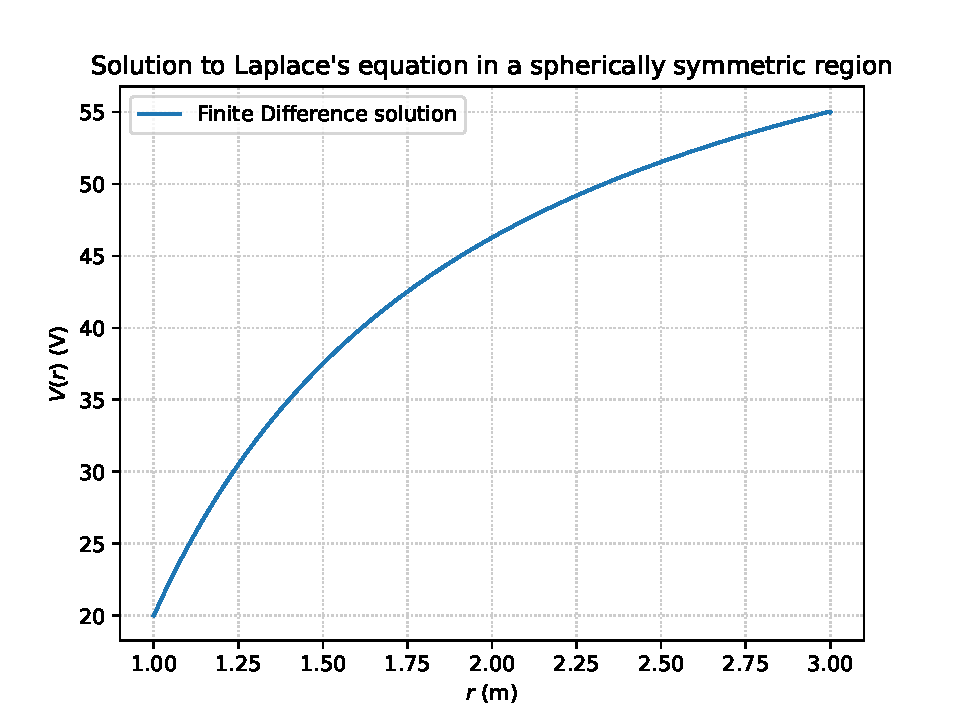
\includegraphics[width=.75\textwidth]{Plots/laplaceFD.pdf}
            \caption{Plot of the solution to \cref{eqn:Laplace} using the linear finite difference method, with $V(r=\SI{1}{\metre})=\SI{20}{\volt}$ and $V(r=\SI{3}{\metre})=\SI{55}{\volt}$. A step of $\Delta r=0.001$ was used. }
            \label{fig:LaplaceFD}
        \end{center}
    \end{figure}

    
    


\end{enumerate}

\end{document}